\documentclass[12pt]{article}

\usepackage{amsmath}
\usepackage{amssymb}
\usepackage{bm}
\usepackage{enumerate}
\usepackage{fancyvrb}
\usepackage[top=1in, bottom=1in, left=1in, right=1in]{geometry}
\usepackage{hyperref}
\usepackage{placeins}
\usepackage{tikz}
\usepackage{tikzsymbols}
\usepackage{todonotes}

\usetikzlibrary{positioning,calc}


%-------------------------------------------------------------------------------
% Custom commands
\usepackage{xcolor} %hilight
\newcommand{\hilight}[1]{\colorbox{yellow}{#1}}
\usepackage[most]{tcolorbox}
\newtcolorbox[]{solution}[1][]{%
    breakable,
    enhanced,
    colback=white,
    title=Solution,
    #1
}
%-------------------------------------------------------------------------------


\title{10-703 Deep RL and Controls\\
  Homework 1\\
  Spring 2018
}

\date{\vspace{-50pt}
\begin{align*}
\text{Released: } & \text{Monday, Feb. 5, 2018} \\
\text{Due: } & \text{Monday, Feb. 19, 2018 @ 11:59:59 PM EST}
\end{align*}
}


\begin{document}

\maketitle

\section*{Instructions}

\noindent Submit the following to Gradescope by Monday, Feb. 19, 11:59:59 PM EST:
\begin{itemize}
\item Your write-up, written in LaTeX and submitted as a PDF file. Handwritten solutions will not be accepted.
\item Your code for Problem 2
\end{itemize}

\noindent You are allowed 7 grace days in total for your homeworks. These do not need to be requested or mentioned in emails; we will automatically apply them to students who submit late. We will not give any further extensions so make sure you only use them when you are absolutely sure you need them. Students who submit late after their grace days have been used will be subject to 10\% of their score for that assignment every additional day used.

\bigskip

\noindent  You can discuss the homework problems with your classmates, but your code and your write-up must be your own. You are expected to comply with the University Policy on Academic Integrity and Plagiarism\footnote{\url{https://www.cmu.edu/policies/}}.

\section*{Problem 1 (13+7=20 pts)}
\label{sec:p1}

Consider an environment in which our agent requires caffeine to function\footnote{If it helps, you can think of the agent as a graduate student.}. Because caffeine is so important to our agent, we would like the agent to find a policy that will always lead it to the shortest path to coffee.

In order to apply optimal control techniques such as value iteration and policy iteration, we first need to model this scenario as a Markov decision process (MDP). Note that there may be many different ways to define each of the MDP components for a given problem. Recall that an MDP is defined as a tuple
$(S, A, P, R, \gamma)$ where:
\begin{description}
\item[$S$] is the (finite) set of all possible states.
\item[$A$] is the (finite) set of all possible actions.
\item[$P$] is the transition function $P: S \times S \times A \to [0, 1]$, 
  which maps $(s', s, a)$ to $P(s'|s, a)$, i.e., 
  the probability of transitioning to state $s'\in S$ when taking action
  $a\in A$ in state $s\in S$. 
  Note that $\sum _{s' \in S} P(s' | s, a) = 1$ for all 
  $s \in S, a \in A$.
\item[$R$] is the reward function $R : S \times A \times S \to \mathbb R$,
which maps $(s, a, s')$ to $R(s, a, s')$, i.e., 
the reward obtained when taking action $a \in A$ in state $s \in S$ and 
arriving at state $s' \in S$.
\item[$\gamma$] is the discount factor, which controls the relative importance of short-term and long-term rewards. We generally have $\gamma \in [0, 1)$, where smaller values mean more discounting of rewards.
\end{description}

For this problem, we represent states by $(x, y, o)$ notation, where $x$ and $y$ are the horizontal and vertical coordinates of the agent's location, respectively, and $o$ is the agent's orientation which is one of $\{ N, E, W, S \}$ (North, East, West, South). The agent's current orientation is the only direction it can move. The agent is able to move forward, turn right, or turn left (deterministically). All actions are available in all states. More specifically, the action space is $|A| = \{F,R,L\}$ where:
\begin{itemize}
\item F (move Forward): The agent moves forward along its current orientation, changing the agent's location but not its orientation.
\item R (turn Right): The agent turns right, changing the agent's orientation but not its location.
\item L (turn Left): The agent turns left, changing the agent's orientation but not its location.
\end{itemize}
Walls are represented by thick black lines. The agent cannot move through walls. If the agent attempts to move through a wall,  it will remain in the same state.

When the agent reaches the coffee cup in any orientation, the episode ends. Another way to think of this is that every action in the coffee cup state keeps the agent in the coffee cup state.

\subsection*{Problem 1, Part I: Markov Decision Process (13 pts)}

\begin{figure}[h]
  \centering
  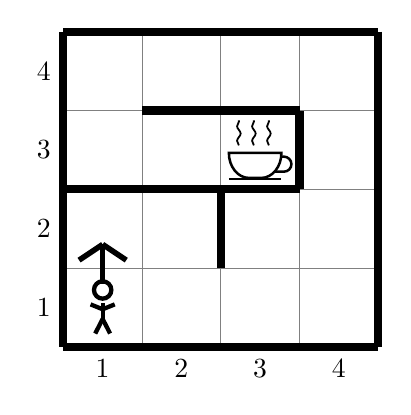
\begin{tikzpicture}
    \draw[step=1cm,gray,very thin] (0,0) grid (4,4);
    \foreach \x in {1, ..., 4}
      \draw (\x cm - .5cm, 1pt) -- (\x cm - .5cm, -1pt)
      node[anchor=north] {$\x$};
      \foreach \y in {1, ..., 4}
      \draw (1pt,\y cm - .5cm) -- (-1pt, \y cm - .5cm)
      node[anchor=east] {$\y$};

      % Agent
      
      \node (agent) at (.5cm, .5cm) {\Strichmaxerl[3]};
      \draw[line width=2pt] (0.5cm, 0.8cm) -- (0.5cm, 1.3cm);
      \draw[line width=2pt] (0.5cm, 1.3cm) -- (0.2cm, 1.1cm);
      \draw[line width=2pt] (0.5cm, 1.3cm) -- (0.8cm, 1.1cm);
      
      % Goal
      \node (goal) at (2.5cm, 2.5cm) {\Coffeecup[3]};

      % Obstacles
      \draw[line width=3pt] (2cm, 1cm) -- (2cm, 2cm);
      \draw[line width=3pt] (0cm, 2cm) -- (3cm, 2cm);
      \draw[line width=3pt] (3cm, 2cm) -- (3cm, 3cm);
      \draw[line width=3pt] (3cm, 3cm) -- (1cm, 3cm);
      \draw[line width=3pt] (4cm, 4cm) -- (4cm, 3cm);

      % Border
      \draw[line width=3pt] (0cm, 0cm) -- (0cm, 4cm);
      \draw[line width=3pt] (0cm, 0cm) -- (4cm, 0cm);
      \draw[line width=3pt] (4cm, 4cm) -- (0cm, 4cm);
      \draw[line width=3pt] (4cm, 4cm) -- (4cm, 0cm);
  \end{tikzpicture}
  \caption{\label{fig:prob1_shortest_path_domain} MDP for Problem 1, Part I. The goal is for the agent to have a policy that always leads it on the shortest path to the coffee at coordinate $(3,3)$. In this instance, the agent's current state is $(1,1, N)$ }
\end{figure}

For this section, consider the instance shown in Figure~\ref{fig:prob1_shortest_path_domain}. The goal, displayed as a coffee cup, is located at $(3,3)$. Using the above problem description answer the following questions:

\begin{enumerate}[a)]
\item  How many states and actions are in this MDP (i.e., what are $|S|$ and $|A|$)? What is the dimensionality of the transition function $P$? (2 pts)

\begin{solution}
States = $4*16 = 64$ \\
Actions = 3 \\
dimensionality of transition function = (\# of states) $\times$ (\# of actions) = $64 \times 64 \times 3 = 12288$
\end{solution}

\item Fill in the probabilities for the transition function $P$. (1 pt)\\
  \begin{center}
    \begin{tabular}{|l|l||c|c|c|c|}\hline
      \multicolumn{2}{|c|}{} &
                               \multicolumn{4}{|c|}{$s'$}\\\hline
      $s$ & $a$ & (1,2,N) & (1,1,S) & (1,4,N) & (1,4,S)\\\hline
      (1,1,S) & F & & & &\\ \hline
      (1,1,N) & F & & & &\\ \hline
      (1,4,E) & R & & & &\\ \hline
    \end{tabular}
  \end{center}

\begin{solution}
\begin{center}
    \begin{tabular}{|l|l||c|c|c|c|}\hline
      \multicolumn{2}{|c|}{} &
                               \multicolumn{4}{|c|}{$s'$}\\\hline
      $s$ & $a$ & (1,2,N) & (1,1,S) & (1,4,N) & (1,4,S)\\\hline
      (1,1,S) & F & 0 & 1 & 0 & 0 \\ \hline
      (1,1,N) & F & 1 & 0 & 0 & 0 \\ \hline
      (1,4,E) & R & 0 & 0 & 0 & 1 \\ \hline
    \end{tabular}
  \end{center}
\end{solution}

\item Describe a reward function $R : S \times A \times S$ and a discount factor $\gamma$ that will lead to an optimal policy giving the shortest path to the coffee cup from all states. Does the value of $\gamma \in (0,1)$ affect the optimal policy in this case? Explain. (2 pts)

\begin{solution}
I will design the reward function such that the agent receives 
\begin{enumerate}
\item reward of "-1", if the next state is not coffee cup
\item reward of "10", if the next step is coffee cup, give
\end{enumerate}

I am choosing to give negative reward for each step not ending at coffee cup to prevent sub=optimal solutions as answer. \\

I will choose $\gamma$ = 1. In fact, I can chose any $\gamma$ value here as it will not change the optimal policy.\\
\end{solution}

\item How many possible deterministic policies are there, including both optimal and non-optimal policies? (2 pts)

\begin{solution}
$3^{64}$
\end{solution}

\item What is an optimal policy for this MDP? Draw the 4 grids (one for each orientation) and label each cell with one of \{F,R,L\}, for Forward, turn Right and turn Left, respectively. Is your policy deterministic or stochastic? (There may be multiple optimal policies. Pick one and show it.) (4 pts)

\begin{solution}
\end{solution}
NORTH
\begin{figure}[h]
  \centering
  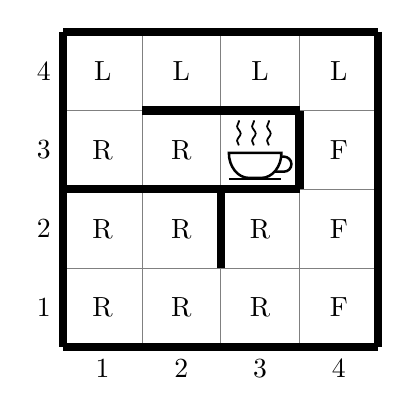
\begin{tikzpicture}
    \draw[step=1cm,gray,very thin] (0,0) grid (4,4);
    \foreach \x in {1, ..., 4}
    \draw (\x cm - .5cm, 1pt) -- (\x cm - .5cm, -1pt)
    node[anchor=north] {$\x$};
    \foreach \y in {1, ..., 4}
    \draw (1pt,\y cm - .5cm) -- (-1pt, \y cm - .5cm)
    node[anchor=east] {$\y$};
      % Agent
      
      % Goal
      \node (goal) at (2.5cm, 2.5cm) {\Coffeecup[3]};

      % Obstacles
      \draw[line width=3pt] (2cm, 1cm) -- (2cm, 2cm);
      \draw[line width=3pt] (0cm, 2cm) -- (3cm, 2cm);
      \draw[line width=3pt] (3cm, 2cm) -- (3cm, 3cm);
      \draw[line width=3pt] (3cm, 3cm) -- (1cm, 3cm);
      \draw[line width=3pt] (4cm, 4cm) -- (4cm, 3cm);

      % Border
      \draw[line width=3pt] (0cm, 0cm) -- (0cm, 4cm);
      \draw[line width=3pt] (0cm, 0cm) -- (4cm, 0cm);
      \draw[line width=3pt] (4cm, 4cm) -- (0cm, 4cm);
      \draw[line width=3pt] (4cm, 4cm) -- (4cm, 0cm);
      
      % Policy
      \node (1) at (.5cm,  .5cm) {R}; % (1,1)
      \node (1) at (1.5cm, .5cm) {R}; % (2,1)
      \node (1) at (2.5cm, .5cm) {R}; % (3,1)
      \node (1) at (3.5cm, .5cm) {F}; % (4,1)
      
      \node (1) at (.5cm,  1.5cm) {R}; % (1,2)
      \node (1) at (1.5cm, 1.5cm) {R}; % (2,2)
      \node (1) at (2.5cm, 1.5cm) {R}; % (3,2)
      \node (1) at (3.5cm, 1.5cm) {F}; % (4,2)
      
      \node (1) at (.5cm,  2.5cm) {R}; % (1,3)
      \node (1) at (1.5cm, 2.5cm) {R}; % (2,3)
      \node (1) at (3.5cm, 2.5cm) {F}; % (4,3)
      
      \node (1) at (.5cm,  3.5cm) {L}; % (1,4)
      \node (1) at (1.5cm, 3.5cm) {L}; % (2,4)
      \node (1) at (2.5cm, 3.5cm) {L}; % (3,4)
      \node (1) at (3.5cm, 3.5cm) {L}; % (4,4)
  \end{tikzpicture}
\end{figure}
\FloatBarrier
SOUTH
\begin{figure}[h]
  \centering
  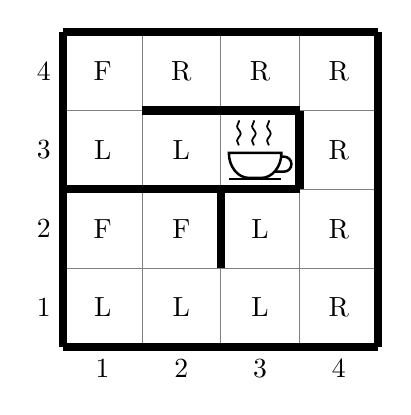
\begin{tikzpicture}
    \draw[step=1cm,gray,very thin] (0,0) grid (4,4);
    \foreach \x in {1, ..., 4}
    \draw (\x cm - .5cm, 1pt) -- (\x cm - .5cm, -1pt)
    node[anchor=north] {$\x$};
    \foreach \y in {1, ..., 4}
    \draw (1pt,\y cm - .5cm) -- (-1pt, \y cm - .5cm)
    node[anchor=east] {$\y$};
      % Agent
      
      % Goal
      \node (goal) at (2.5cm, 2.5cm) {\Coffeecup[3]};

      % Obstacles
      \draw[line width=3pt] (2cm, 1cm) -- (2cm, 2cm);
      \draw[line width=3pt] (0cm, 2cm) -- (3cm, 2cm);
      \draw[line width=3pt] (3cm, 2cm) -- (3cm, 3cm);
      \draw[line width=3pt] (3cm, 3cm) -- (1cm, 3cm);
      \draw[line width=3pt] (4cm, 4cm) -- (4cm, 3cm);

      % Border
      \draw[line width=3pt] (0cm, 0cm) -- (0cm, 4cm);
      \draw[line width=3pt] (0cm, 0cm) -- (4cm, 0cm);
      \draw[line width=3pt] (4cm, 4cm) -- (0cm, 4cm);
      \draw[line width=3pt] (4cm, 4cm) -- (4cm, 0cm);
      
      % Policy
      \node (1) at (.5cm,  .5cm) {L}; % (1,1)
      \node (1) at (1.5cm, .5cm) {L}; % (2,1)
      \node (1) at (2.5cm, .5cm) {L}; % (3,1)
      \node (1) at (3.5cm, .5cm) {R}; % (4,1)
      
      \node (1) at (.5cm,  1.5cm) {F}; % (1,2)
      \node (1) at (1.5cm, 1.5cm) {F}; % (2,2)
      \node (1) at (2.5cm, 1.5cm) {L}; % (3,2)
      \node (1) at (3.5cm, 1.5cm) {R}; % (4,2)
      
      \node (1) at (.5cm,  2.5cm) {L}; % (1,3)
      \node (1) at (1.5cm, 2.5cm) {L}; % (2,3)
      \node (1) at (3.5cm, 2.5cm) {R}; % (4,3)
      
      \node (1) at (.5cm,  3.5cm) {F}; % (1,4)
      \node (1) at (1.5cm, 3.5cm) {R}; % (2,4)
      \node (1) at (2.5cm, 3.5cm) {R}; % (3,4)
      \node (1) at (3.5cm, 3.5cm) {R}; % (4,4)
  \end{tikzpicture}
\end{figure}
\FloatBarrier
EAST
\begin{figure}[h]
  \centering
  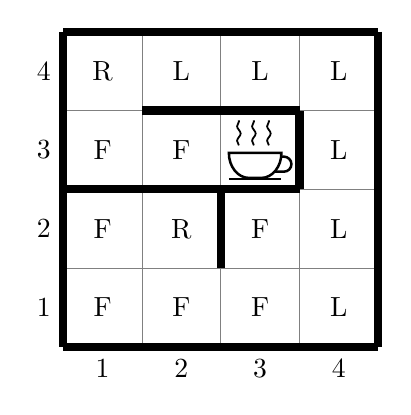
\begin{tikzpicture}
    \draw[step=1cm,gray,very thin] (0,0) grid (4,4);
    \foreach \x in {1, ..., 4}
    \draw (\x cm - .5cm, 1pt) -- (\x cm - .5cm, -1pt)
    node[anchor=north] {$\x$};
    \foreach \y in {1, ..., 4}
    \draw (1pt,\y cm - .5cm) -- (-1pt, \y cm - .5cm)
    node[anchor=east] {$\y$};
      % Agent
      
      % Goal
      \node (goal) at (2.5cm, 2.5cm) {\Coffeecup[3]};

      % Obstacles
      \draw[line width=3pt] (2cm, 1cm) -- (2cm, 2cm);
      \draw[line width=3pt] (0cm, 2cm) -- (3cm, 2cm);
      \draw[line width=3pt] (3cm, 2cm) -- (3cm, 3cm);
      \draw[line width=3pt] (3cm, 3cm) -- (1cm, 3cm);
      \draw[line width=3pt] (4cm, 4cm) -- (4cm, 3cm);

      % Border
      \draw[line width=3pt] (0cm, 0cm) -- (0cm, 4cm);
      \draw[line width=3pt] (0cm, 0cm) -- (4cm, 0cm);
      \draw[line width=3pt] (4cm, 4cm) -- (0cm, 4cm);
      \draw[line width=3pt] (4cm, 4cm) -- (4cm, 0cm);
      
      % Policy
      \node (1) at (.5cm,  .5cm) {F}; % (1,1)
      \node (1) at (1.5cm, .5cm) {F}; % (2,1)
      \node (1) at (2.5cm, .5cm) {F}; % (3,1)
      \node (1) at (3.5cm, .5cm) {L}; % (4,1)
      
      \node (1) at (.5cm,  1.5cm) {F}; % (1,2)
      \node (1) at (1.5cm, 1.5cm) {R}; % (2,2)
      \node (1) at (2.5cm, 1.5cm) {F}; % (3,2)
      \node (1) at (3.5cm, 1.5cm) {L}; % (4,2)
      
      \node (1) at (.5cm,  2.5cm) {F}; % (1,3)
      \node (1) at (1.5cm, 2.5cm) {F}; % (2,3)
      \node (1) at (3.5cm, 2.5cm) {L}; % (4,3)
      
      \node (1) at (.5cm,  3.5cm) {R}; % (1,4)
      \node (1) at (1.5cm, 3.5cm) {L}; % (2,4)
      \node (1) at (2.5cm, 3.5cm) {L}; % (3,4)
      \node (1) at (3.5cm, 3.5cm) {L}; % (4,4)
  \end{tikzpicture}
\end{figure}
\FloatBarrier
WEST
\begin{figure}[h]
  \centering
  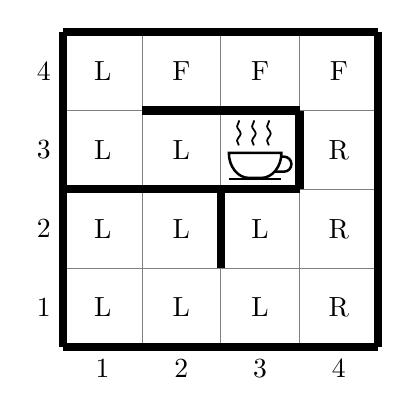
\begin{tikzpicture}
    \draw[step=1cm,gray,very thin] (0,0) grid (4,4);
    \foreach \x in {1, ..., 4}
    \draw (\x cm - .5cm, 1pt) -- (\x cm - .5cm, -1pt)
    node[anchor=north] {$\x$};
    \foreach \y in {1, ..., 4}
    \draw (1pt,\y cm - .5cm) -- (-1pt, \y cm - .5cm)
    node[anchor=east] {$\y$};
      % Agent
      
      % Goal
      \node (goal) at (2.5cm, 2.5cm) {\Coffeecup[3]};

      % Obstacles
      \draw[line width=3pt] (2cm, 1cm) -- (2cm, 2cm);
      \draw[line width=3pt] (0cm, 2cm) -- (3cm, 2cm);
      \draw[line width=3pt] (3cm, 2cm) -- (3cm, 3cm);
      \draw[line width=3pt] (3cm, 3cm) -- (1cm, 3cm);
      \draw[line width=3pt] (4cm, 4cm) -- (4cm, 3cm);

      % Border
      \draw[line width=3pt] (0cm, 0cm) -- (0cm, 4cm);
      \draw[line width=3pt] (0cm, 0cm) -- (4cm, 0cm);
      \draw[line width=3pt] (4cm, 4cm) -- (0cm, 4cm);
      \draw[line width=3pt] (4cm, 4cm) -- (4cm, 0cm);
      
      % Policy
      \node (1) at (.5cm,  .5cm) {L}; % (1,1)
      \node (1) at (1.5cm, .5cm) {L}; % (2,1)
      \node (1) at (2.5cm, .5cm) {L}; % (3,1)
      \node (1) at (3.5cm, .5cm) {R}; % (4,1)
      
      \node (1) at (.5cm,  1.5cm) {L}; % (1,2)
      \node (1) at (1.5cm, 1.5cm) {L}; % (2,2)
      \node (1) at (2.5cm, 1.5cm) {L}; % (3,2)
      \node (1) at (3.5cm, 1.5cm) {R}; % (4,2)
      
      \node (1) at (.5cm,  2.5cm) {L}; % (1,3)
      \node (1) at (1.5cm, 2.5cm) {L}; % (2,3)
      \node (1) at (3.5cm, 2.5cm) {R}; % (4,3)
      
      \node (1) at (.5cm,  3.5cm) {L}; % (1,4)
      \node (1) at (1.5cm, 3.5cm) {F}; % (2,4)
      \node (1) at (2.5cm, 3.5cm) {F}; % (3,4)
      \node (1) at (3.5cm, 3.5cm) {F}; % (4,4)
  \end{tikzpicture}
\end{figure}
\FloatBarrier
\item Is there any advantage to having a stochastic policy for this MDP? Explain. In general, what are the advantages of using a stochastic policy? (2 pts)

\begin{solution}
For this MDP there is no advantage to having stochastic policy. Here the model of the system is known (fully) and there is no uncertainty in the system so a deterministic policy works well.

Stochastic policy is good where the model of the system is not fully known or if we want to do model free learning. Also in case of uncertainty and hidden states, stochastic policy will be more robust. Deterministic policy on the other hand will model the average behavior of the system. 

\end{solution}

\end{enumerate}

\subsection*{Problem 1, Part II: Reward and Discount Factor (7 pts)}

In this section, consider the instance in Fig.~\ref{fig:1b-mdp}. This time, the agent has a choice between (1) a small coffee closer to the agent and (2) a large coffee further away from the agent. We will use this scenario to explore the interaction between optimal policy, discount factor, and reward function. Again, each coffee cup is still an absorbing state: when the agent reaches one of the coffee cups, the episode ends.

\begin{figure}[h]
  \centering
  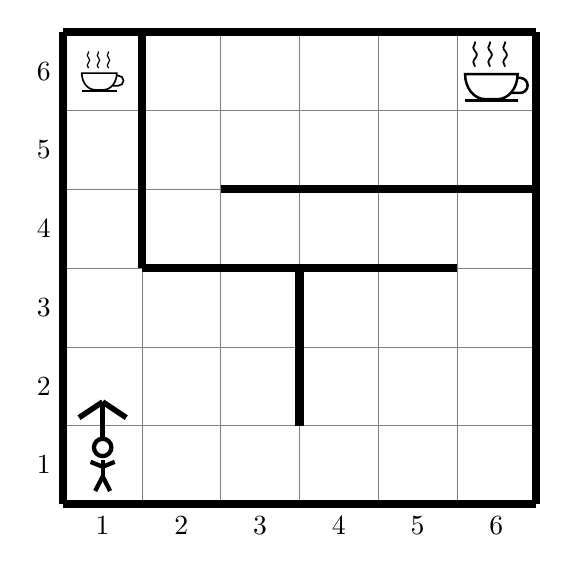
\begin{tikzpicture}
    % draw the grid and label the edges
    \draw[step=1cm,gray,very thin] (0,0) grid (6,6);
    \foreach \x in {1, ..., 6}
      \draw (\x cm - .5cm, 1pt) -- (\x cm - .5cm, -1pt)
      node[anchor=north] {$\x$};
      \foreach \y in {1, ..., 6}
      \draw (1pt,\y cm - .5cm) -- (-1pt, \y cm - .5cm)
      node[anchor=east] {$\y$};

      %\draw[fill=green, fill opacity=.2] (0cm, 6cm) -- (6cm,6cm) --
      (6cm, 4cm) -- (1cm, 4cm) -- (1cm, 5cm) -- (0cm, 5cm) -- cycle;

      %\draw[fill=blue, fill opacity=.2] (0cm, 5cm) -- (1cm, 5cm) --
      (1cm, 4cm) -- (6cm, 4cm) -- (6cm, 0cm) -- (0cm, 0cm) -- cycle;

      % Agent
      \node (agent) at (.5cm, .5cm) {\Strichmaxerl[3]};
      \draw[line width=2pt] (0.5cm, 0.8cm) -- (0.5cm, 1.3cm);
      \draw[line width=2pt] (0.5cm, 1.3cm) -- (0.2cm, 1.1cm);
      \draw[line width=2pt] (0.5cm, 1.3cm) -- (0.8cm, 1.1cm);
      
      % Goal
      \node (goal) at (5.5cm, 5.5cm) {\Coffeecup[3]};
      \node (goal) at (.5cm, 5.5cm) {\Coffeecup[2]};

      % Obstacles
      \draw[line width=3pt] (1cm, 3cm) -- (5cm, 3cm);
      \draw[line width=3pt] (3cm, 3cm) -- (3cm, 1cm);

      \draw[line width=3pt] (2cm, 4cm) -- (6cm, 4cm);
      \draw[line width=3pt] (1cm, 3cm) -- (1cm, 6cm);
  
      % Border
      \draw[line width=3pt] (0cm, 0cm) -- (0cm, 6cm);
      \draw[line width=3pt] (0cm, 0cm) -- (6cm, 0cm);
      \draw[line width=3pt] (6cm, 6cm) -- (0cm, 6cm);
      \draw[line width=3pt] (6cm, 6cm) -- (6cm, 0cm);
  \end{tikzpicture}
  \caption{MDP for Problem 1, Part II. The agent starts in state $(1, 1, N)$. This time, the agent has a choice between a small coffee at $(1,6)$ closer to the agent and a large coffee at $(6,6)$ further away from the agent. \label{fig:1b-mdp}}
\end{figure}
\FloatBarrier

\begin{enumerate}[a)]
\item For a fixed reward function of +10 for the large coffee, +1 for the small coffee and 0 elsewhere, describe the optimal policy behavior for each value of the discount factor $\gamma$. (2 pts)

\begin{solution}
For the case  when agent is starting at (1, 1, N) and there is no penalty on time (number of steps), the value of state is $max(\gamma^{n_{small} -1} \times 1, \gamma^{n_{large} -1} \times 10)$; where $n_{small} and n_{large}$ are the minimum number of steps that the agent can take to reach the small coffee and large coffee respectively\\
From start state to small coffee, the agent needs to take at least 5 steps. Similarly from start state to large coffee, the agent needs to take at least 23 steps.\\
So the agent will go to small coffee if:
\begin{align} 
\gamma^4 \time 1 &> \gamma^{22} \times 10 \\
\gamma &< 0.1^{\frac{1}{18}}\\
\gamma &< 0.8799
\end{align}

\begin{enumerate}
\item $\gamma < 0.8799$, the agent will follow this policy: $F \rightarrow F \rightarrow F \rightarrow F \rightarrow F$
\item $\gamma > 0.8799$, the agent will follow this policy: $R \rightarrow F \rightarrow F \rightarrow F \rightarrow F \rightarrow F \rightarrow L \rightarrow F \rightarrow F \rightarrow F \rightarrow L \rightarrow F \rightarrow F \rightarrow F \rightarrow R \rightarrow F \rightarrow F \rightarrow R \rightarrow F \rightarrow F \rightarrow F$
\item $\gamma = 0.8799$, the agent is neutral towards goal position and will follow either of the above two policies with 50\% probability.
\end{enumerate}
\end{solution}

\begin{figure}[h]
  \centering
  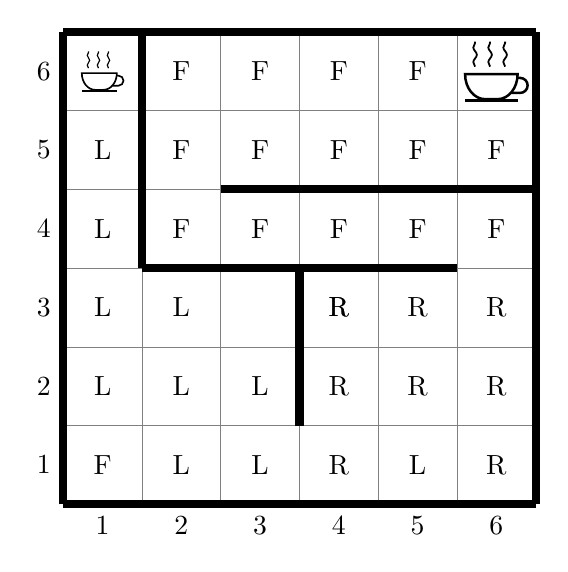
\begin{tikzpicture}
    % draw the grid and label the edges
    \draw[step=1cm,gray,very thin] (0,0) grid (6,6);
    \foreach \x in {1, ..., 6}
      \draw (\x cm - .5cm, 1pt) -- (\x cm - .5cm, -1pt)
      node[anchor=north] {$\x$};
      \foreach \y in {1, ..., 6}
      \draw (1pt,\y cm - .5cm) -- (-1pt, \y cm - .5cm)
      node[anchor=east] {$\y$};

      %\draw[fill=green, fill opacity=.2] (0cm, 6cm) -- (6cm,6cm) --
      (6cm, 4cm) -- (1cm, 4cm) -- (1cm, 5cm) -- (0cm, 5cm) -- cycle;

      %\draw[fill=blue, fill opacity=.2] (0cm, 5cm) -- (1cm, 5cm) --
      (1cm, 4cm) -- (6cm, 4cm) -- (6cm, 0cm) -- (0cm, 0cm) -- cycle;
      
      % Goal
      \node (goal) at (5.5cm, 5.5cm) {\Coffeecup[3]};
      \node (goal) at (.5cm, 5.5cm) {\Coffeecup[2]};

      % Obstacles
      \draw[line width=3pt] (1cm, 3cm) -- (5cm, 3cm);
      \draw[line width=3pt] (3cm, 3cm) -- (3cm, 1cm);

      \draw[line width=3pt] (2cm, 4cm) -- (6cm, 4cm);
      \draw[line width=3pt] (1cm, 3cm) -- (1cm, 6cm);
  
      % Border
      \draw[line width=3pt] (0cm, 0cm) -- (0cm, 6cm);
      \draw[line width=3pt] (0cm, 0cm) -- (6cm, 0cm);
      \draw[line width=3pt] (6cm, 6cm) -- (0cm, 6cm);
      \draw[line width=3pt] (6cm, 6cm) -- (6cm, 0cm);
      
      % Policy
        \node (1) at (.5cm,  .5cm) {F}; % (1,1)
        \node (1) at (1.5cm, .5cm) {L}; % (2,1)
        \node (1) at (2.5cm, .5cm) {L}; % (3,1)
        \node (1) at (3.5cm, .5cm) {R}; % (4,1)
        \node (1) at (4.5cm, .5cm) {L}; % (5,1)
        \node (1) at (5.5cm, .5cm) {R}; % (6,1)
        
        \node (1) at (.5cm,  1.5cm) {L}; % (1,2)
        \node (1) at (1.5cm, 1.5cm) {L}; % (2,2)
        \node (1) at (2.5cm, 1.5cm) {L}; % (3,2)
        \node (1) at (3.5cm, 1.5cm) {R}; % (4,2)
        \node (1) at (4.5cm, 1.5cm) {R}; % (5,2)
        \node (1) at (5.5cm, 1.5cm) {R}; % (6,2)
        
        \node (1) at (.5cm,  2.5cm) {L}; % (1,3)
        \node (1) at (1.5cm, 2.5cm) {L}; % (2,3)
        \node (1) at (3.5cm, 2.5cm) {R}; % (4,3)
        \node (1) at (3.5cm, 2.5cm) {R}; % (4,3)
        \node (1) at (4.5cm, 2.5cm) {R}; % (5,3)
        \node (1) at (5.5cm, 2.5cm) {R}; % (6,3)
        
        \node (1) at (.5cm,  3.5cm) {L}; % (1,4)
        \node (1) at (1.5cm, 3.5cm) {F}; % (2,4)
        \node (1) at (2.5cm, 3.5cm) {F}; % (3,4)
        \node (1) at (3.5cm, 3.5cm) {F}; % (4,4)
        \node (1) at (4.5cm, 3.5cm) {F}; % (5,4)
        \node (1) at (5.5cm, 3.5cm) {F}; % (6,4)
        
        \node (1) at (.5cm,  4.5cm) {L}; % (1,4)
        \node (1) at (1.5cm, 4.5cm) {F}; % (2,4)
        \node (1) at (2.5cm, 4.5cm) {F}; % (3,4)
        \node (1) at (3.5cm, 4.5cm) {F}; % (4,4)
        \node (1) at (4.5cm, 4.5cm) {F}; % (5,4)
        \node (1) at (5.5cm, 4.5cm) {F}; % (6,4)
        
        \node (1) at (1.5cm, 5.5cm) {F}; % (2,4)
        \node (1) at (2.5cm, 5.5cm) {F}; % (3,4)
        \node (1) at (3.5cm, 5.5cm) {F}; % (4,4)
        \node (1) at (4.5cm, 5.5cm) {F}; % (5,4)
  \end{tikzpicture}
  \caption{MDP for Problem 1, Part II. The agent starts in state $(1, 1, N)$. This time, the agent has a choice between a small coffee at $(1,6)$ closer to the agent and a large coffee at $(6,6)$ further away from the agent. \label{fig:1b-mdp}}
\end{figure}
\FloatBarrier

\item Suppose the discount factor is $\gamma = 1$ and the reward function gives +10 for the large coffee and +1 for the small coffee. Here we will add a negative reward $r < 0$ to every action the agent takes (think of it as a penalty for using energy). Describe the optimal policy behavior for each value of $r$. (2 pts)

\begin{solution}
Considering the case when agent is starting at (1, 1, N), there is negative reward to every action and $\gamma = 1$. The value of state is $ max((n_{small}-1) \times r + 1, (n_{large}-1) \times r + 10)$; where $n_{small} and n_{large}$ are the minimum number of steps that the agent can take to reach the small coffee and large coffee respectively\\
From start state to small coffee, the agent needs to take at least 5 steps. Similarly from start state to large coffee, the agent needs to take at least 23 steps.\\
So the agent will go to small coffee if:
\begin{align} 
4\times r + 1 &> 22 \times r + 10 \\
18\times r &< -9\\
r &< -0.5
\end{align}
\begin{enumerate}
\item $r < -0.5$, the agent will follow this policy: $F \rightarrow F \rightarrow F \rightarrow F \rightarrow F$
\item $r > -0.5$ and $r < 0$, the agent will follow this policy: $R \rightarrow F \rightarrow F \rightarrow F \rightarrow F \rightarrow F \rightarrow L \rightarrow F \rightarrow F \rightarrow F \rightarrow L \rightarrow F \rightarrow F \rightarrow F \rightarrow R \rightarrow F \rightarrow F \rightarrow R \rightarrow F \rightarrow F \rightarrow F$
\item  $r = -0.5$, the agent is neutral towards goal position and will follow either of the above two policies with 50\% probability.
\end{enumerate}
\end{solution}

\item What would happen to the optimal policy if we chose $r$ to be a positive number in the previous question? (1 pts)

\begin{solution}
The problem will become infinite horizon and will not converge. The agent will keep moving in the grid and keep collecting the reward but will never terminate.
\end{solution}

\item For a fixed discount factor of 0.9, find a reward function for which the optimal policy will prefer going to the small coffee from the starting state, and a reward function for which the optimal policy will prefer going to the large coffee from the starting state. (2 pts)

\begin{solution}
For the case  when agent is starting at (1, 1, N) and let's assume there is no penalty on taking actions, the value of state is $max(\gamma^{n_{small} -1} \times r_{small}, \gamma^{n_{large} -1} \times r_{large})$; where $n_{small} and n_{large}$ are the minimum number of steps that the agent can take to reach the small coffee and large coffee respectively and $r_{small} and r_{large}$ are the end rewards for getting small coffee and large coffee respectively\\
From start state to small coffee, the agent needs to take at least 5 steps. Similarly from start state to large coffee, the agent needs to take at least 23 steps.\\
So the agent will go to small coffee if:
\begin{align} 
\gamma^4 \times r_{small} &> \gamma^{22} \times r_{large} \\
Let r_{small} = 1 \\
\frac{1}{0.9^{18}} &> r_{large}\\
r_{large} &< 6.66
\end{align}

Hence, to prefer small coffee, I will assign zero reward for taking action and +1 for getting small coffee and +6 for getting large coffee\\

To prefer large coffee, I will assign zero reward for taking action and +1 for small coffee and +10 for large coffee.
%Considering To prefer going to small coffee at $\gamma = 0.9$ we can have negative reward $r$ for taking action. To find the value of $r$, use the equations similar to part b as:
%To prefer going to large coffee, we can simply have 0 reward for taking action and as proved in part a, the agent will prefer to go to large coffee.
\end{solution}

\end{enumerate}

\section*{Problem 2 (37+10+8=55 pts)}

In this problem, you will implement value iteration and policy iteration. We will be working with different versions of the OpenAI Gym FrozenLake environment\footnote{\url{https://gym.openai.com/envs/FrozenLake-v0}}, defined in \\
\texttt{deeprl\_hw1/lake\_envs.py}. Specific coding instructions are provided in the source code and \texttt{README.md}. Function templates are provided in \texttt{deeprl\_hw1/rl.py} for you to fill in. You may use either Python 2.7 or Python 3. 

In this domain , the agent starts at a fixed starting position, marked with ``S''. The agent can move up, down, left, and right.
\begin{itemize}
\item In the deterministic environments (\texttt{Deterministic-*-FrozenLake-v0}), the up action will always move the agent up, the left will always move left, etc.
\item In the stochastic environments (\texttt{Stochastic-*-FrozenLake-v0}), the ice is slippery, so the agent won't always move in the direction it intends. Specifically, each action will move the agent in the intended direction with probability $\frac{1}{3}$, to the right of the intended direction with probability $\frac{1}{3}$, and to the left of the intended direction with probability $\frac{1}{3}$.
\end{itemize}

We have provided two different maps, a $4 \times 4$ map and a $8 \times 8$ map:
\begin{center}
  \begin{minipage}[c]{0.3\textwidth}
    \begin{BVerbatim}
        GHFS
        FHHF
        FFHF
        FFFF
    \end{BVerbatim}
\end{minipage}%
%
\begin{minipage}[c]{0.3\textwidth}
    \begin{BVerbatim}
        FFFSFFFF
        FFFFFFFF
        HHHHFHFF
        FFFFFFHF
        FFFFFFFF
        FHFFFFHF
        FHFFHFHH
        FGHFFFFF
    \end{BVerbatim}
\end{minipage}%
\end{center}
There are four different tile types: Start (S), Frozen (F), Hole (H), and Goal (G).
\begin{itemize}
\item The agent starts in the Start tile at the beginning of each episode.
\item When the agent lands on a Frozen or Start tile, it receives {\color{red} $0$} reward.
\item When the agent lands on a Hole tile, it receives $0$ reward and the episode ends.
\item When the agent lands on the Goal tile, it receives $+1$ reward and the episode ends.
\end{itemize}

States are represented as integers numbered from left to right, top to bottom starting at zero. For example in a $4\times 4$ map, the upper-left corner is state $0$ and the bottom-right corner is state $15$:
\begin{center}\begin{tabular}{cccc}
0 & 1 & 2 & 3 \\
4 & 5 & 6 & 7 \\
8 & 9 & 10 & 11 \\
12 & 13 & 14 & 15
\end{tabular}\end{center}

\textbf{Note:} Be careful when implementing value iteration and policy evaluation. Keep in mind that in this environment, the reward function depends on the current state, the current action, and the \textbf{next state}. Also, terminal states are slightly different. Think about the backup diagram for terminal states and how that will affect the Bellman equation.

\begin{center}\begin{figure}[h!]
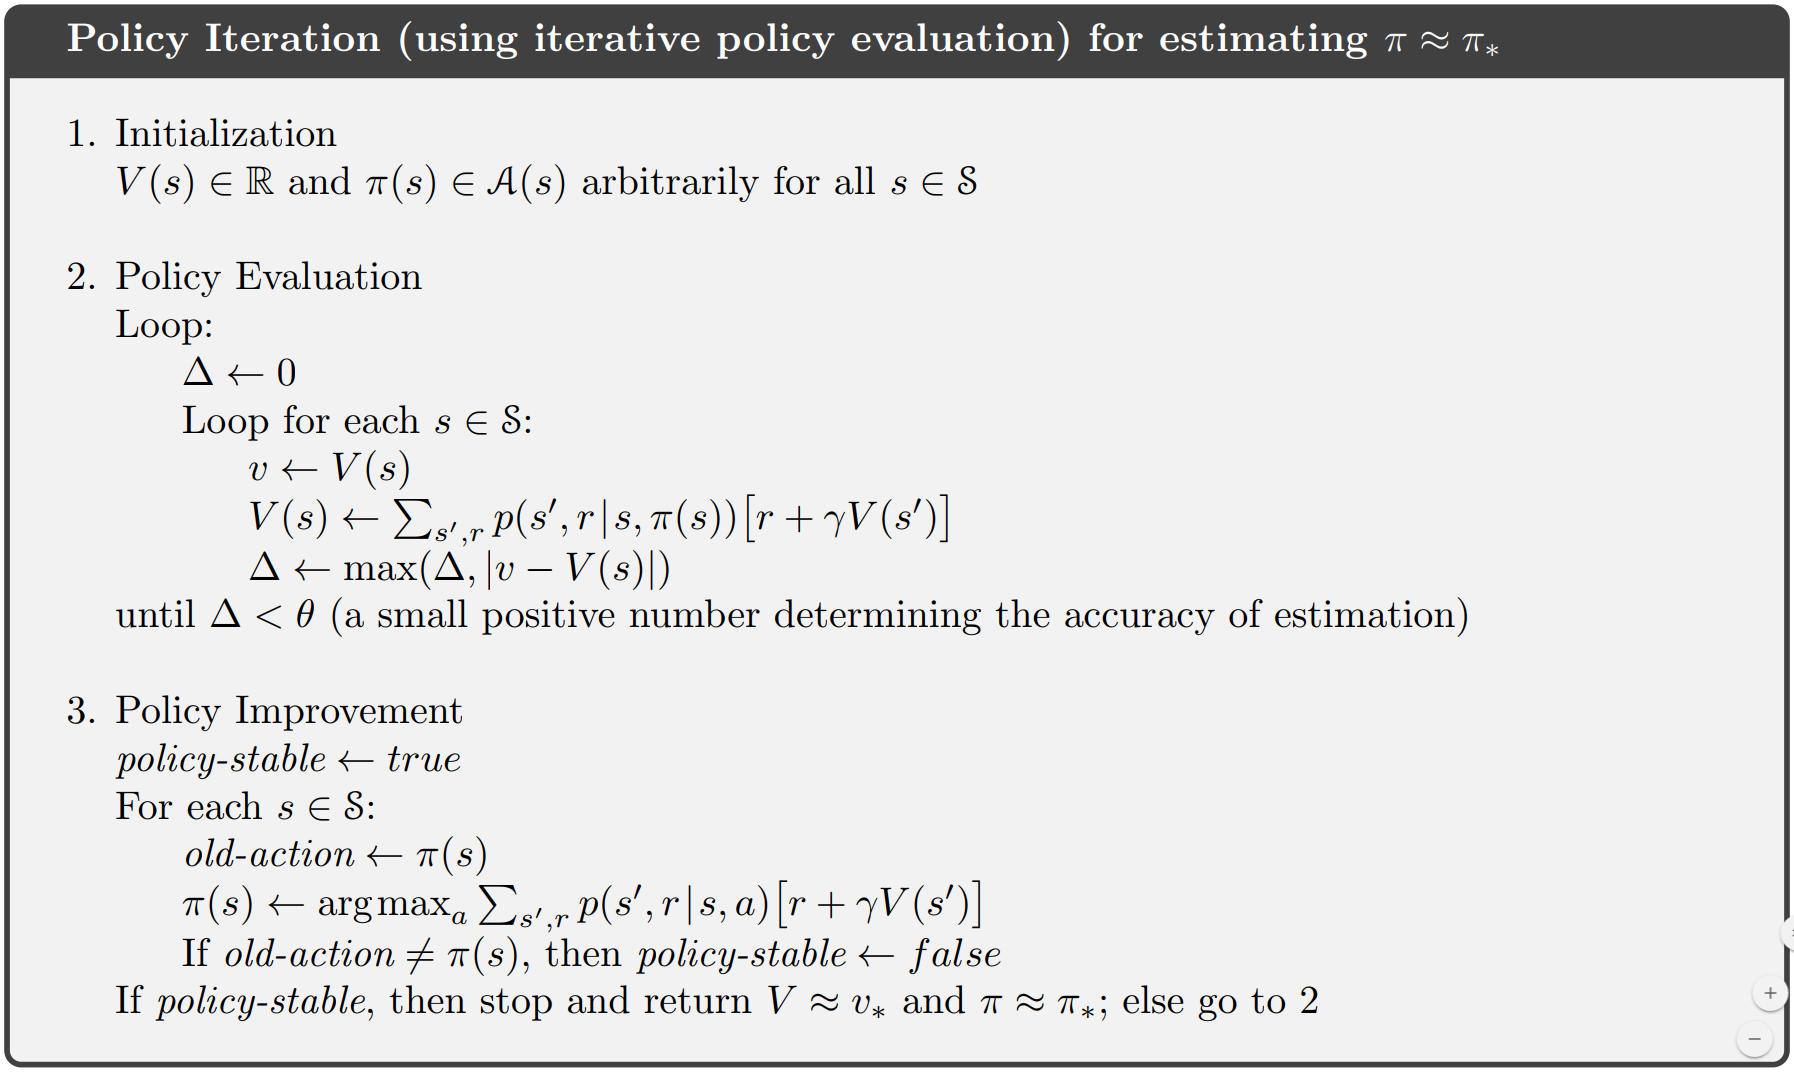
\includegraphics[width=\textwidth]{figures/policy-iteration.png}
\caption{Policy iteration, taken from Section 4.3 of Sutton \& Barto's RL book (2018).\label{fig:policy-iteration}}
\vspace{15pt}
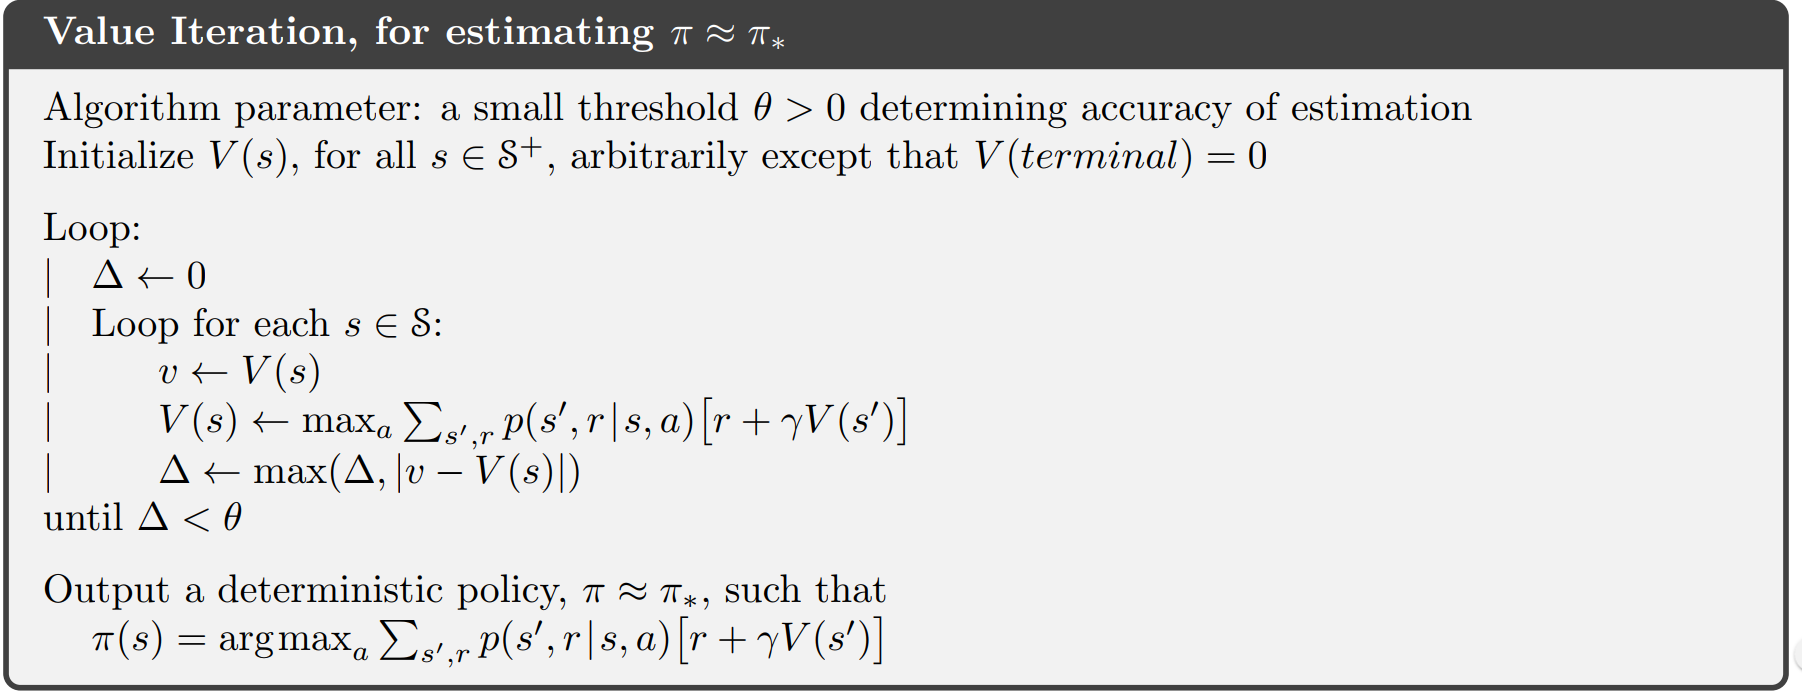
\includegraphics[width=\textwidth]{figures/value-iteration.png}
\caption{Value iteration, taken from Section 4.4 of Sutton \& Barto's RL book (2018).\label{fig:value-iteration}}
\end{figure}
\end{center}

\subsection*{Problem 2, Part I: Deterministic Environment (37 pts)}

In this section, we will use the deterministic versions of the FrozenLake environment. Answer the following questions for the maps
\texttt{Deterministic-4x4-FrozenLake-v0} and\\ \texttt{Deterministic-8x8-FrozenLake-v0}.

\begin{enumerate}[a)]
\item Find the optimal policy using \textbf{synchronous policy iteration}. Specifically, you will implement \texttt{policy\_iteration\_sync()} in \texttt{deeprl\_hw1/rl.py}, writing the policy evaluation and policy improvement steps in \texttt{evaluate\_policy\_sync()} and \texttt{improve\_policy()}, respectively. Record (1) the time taken for execution, (2) the number of policy improvement steps, and (3) the total number of policy evaluation steps. Use a discount factor of $\gamma=0.9$. Use a stopping tolerance of $\theta = 10^{-3}$ for the policy evaluation step. (5 pts)

\begin{center}
  \begin{tabular}{|c|c|c|c|}\hline
    {\bf Environment} & {\bf Time (ms)} & {\bf \shortstack{\# Policy \\ Improvement \\ Steps}} & {\bf \shortstack{Total \# \\ Policy \\ Evaluation \\ Steps}} \\ \hline
    Deterministic-4x4 & & & \\ \hline
    Deterministic-8x8 & & & \\ \hline
  \end{tabular}
\end{center}

\begin{solution}
\begin{center}
  \begin{tabular}{|c|c|c|c|}\hline
    {\bf Environment} & {\bf Time (ms)} & {\bf \shortstack{\# Policy \\ Improvement \\ Steps}} & {\bf \shortstack{Total \# \\ Policy \\ Evaluation \\ Steps}} \\ \hline
    Deterministic-4x4 & 5.4 & 8 & 52 \\ \hline
    Deterministic-8x8 & 29.8 & 13 & 145 \\ \hline
  \end{tabular}
\end{center}
\end{solution}

\item What is the optimal policy for this map? Show as a grid of letters with ``U'', ``D'', ``L'', ``R'' representing the actions up, down, left, right respectively. See Figure~\ref{fig:prob2_example_policy} for an example of the expected output. (3 pts)

\begin{figure}[ht]
  \centering
  \begin{BVerbatim}
LLLL
DDDD
UUUU
RRRR
  \end{BVerbatim}
  \caption{\label{fig:prob2_example_policy} An example (deterministic) policy for a $4 \times 4$ map of the \texttt{FrozenLake-v0} environment. L, D, U, R represent the actions up, down, left, right respectively.}
\end{figure}

\begin{solution}
For 4x4 map: \\
LLRD \\
ULLD \\
ULLD \\
ULLL \\ \\%
For 8x8 map: \\
DDDDDLLL \\
RRRRDLLL \\
LLLLDLRD \\
DLLLLLLD \\
DLLLLLLL \\
DLULLLLU \\
DLULLULL \\
RLLULLLL
\end{solution}

\item Find the value function of this policy. Plot it as a color image, where each square shows its value as a color. See Figure~\ref{fig:prob3_value_image} for an example. (3 pts)

\begin{figure}[h]
  \centering
  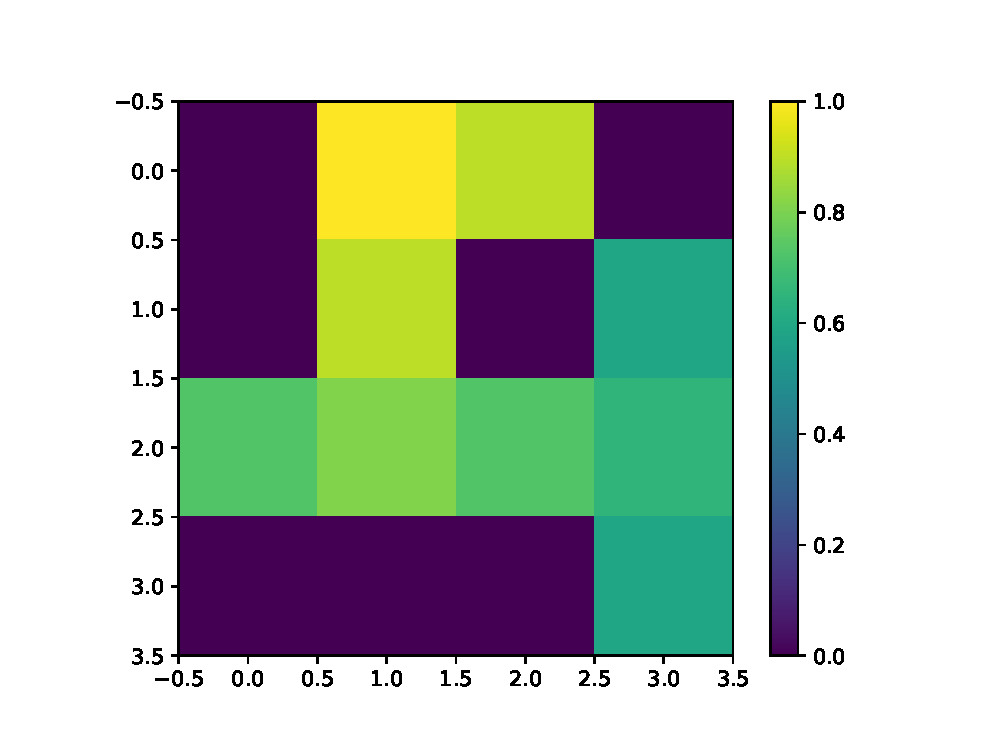
\includegraphics[width=.5\textwidth]{figures/value_function_plot.eps}
  \caption{\label{fig:prob3_value_image} Example of value function
    color plot for a $4 \times 4$ map of the \texttt{FrozenLake-v0} environment. Make sure you include the color bar or some kind of key.}
\end{figure}

\begin{solution}
4X4: Figure~\ref{fig:prob3_value_image_solution_for_policy_iteration}\\
8X8: Figure~\ref{fig:prob3_value_image_solution_for_policy_iteration_8X8}
\end{solution}
\begin{figure}[h]
  \centering
  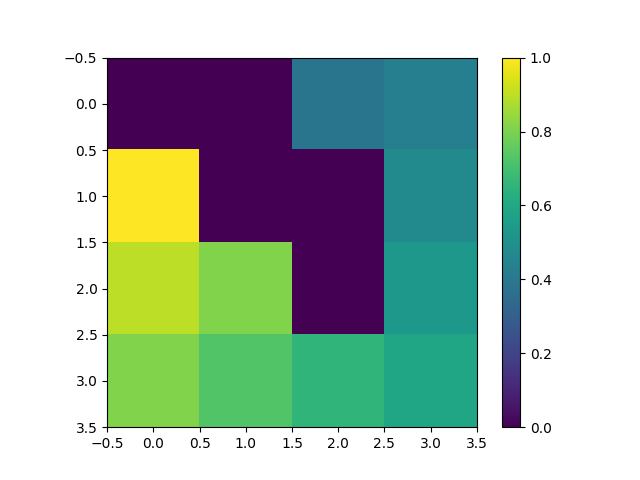
\includegraphics[width=.5\textwidth]{figures/sync_policy_iteration_value_map.png}
  \caption{\label{fig:prob3_value_image_solution_for_policy_iteration} Solution of value function color plot for a $4 \times 4$ map of the \texttt{FrozenLake-v0} environment.}
\end{figure}
\FloatBarrier

\begin{figure}[h]
  \centering
  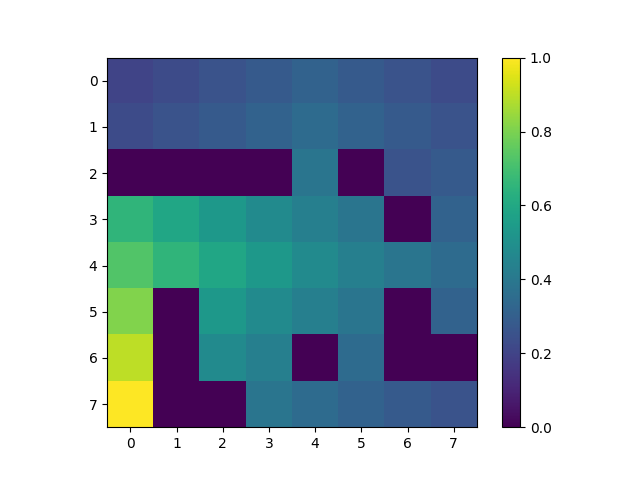
\includegraphics[width=.5\textwidth]{figures/8X8_sync_policy_iteration_value_map.png}
  \caption{\label{fig:prob3_value_image_solution_for_policy_iteration_8X8} Solution of value function color plot for a $8 \times 8$ map of the \texttt{FrozenLake-v0} environment.}
\end{figure}
\FloatBarrier

\item Find the optimal value function directly using \textbf{synchronous value iteration}. Specifically, you will implement \texttt{value\_iteration\_sync()} in \texttt{deeprl\_hw1/rl.py}. Record the time taken for execution, and the number of iterations it took to converge. Use $\gamma=0.9$ Use a stopping tolerance of $10^{-3}$. (5 pts)

\begin{center}
  \begin{tabular}{|c|c|c|}\hline
    {\bf Environment} & {\bf Time (ms)} & {\bf \# Iterations} \\ \hline
    Deterministic-4x4 & & \\ \hline
    Deterministic-8x8 & & \\ \hline
  \end{tabular}
\end{center}

\begin{solution}
\begin{center}
  \begin{tabular}{|c|c|c|}\hline
    {\bf Environment} & {\bf Time (ms)} & {\bf \# Iterations} \\ \hline
    Deterministic-4x4 & 1.16 & 11 \\ \hline
    Deterministic-8x8 & 6.65 & 17 \\ \hline
  \end{tabular}
\end{center}
\end{solution}

\item Plot this value function as a color image, where each square shows its value as a color. See Figure~\ref{fig:prob3_value_image} for an example. (3 pts)

\begin{solution}
4X4: Figure~\ref{fig:prob3_value_image_solution_for_value_iteration} \\
8X8: Figure~\ref{fig:prob3_value_image_solution_for_value_iteration_8X8}
\end{solution}

\begin{figure}[h]
  \centering
  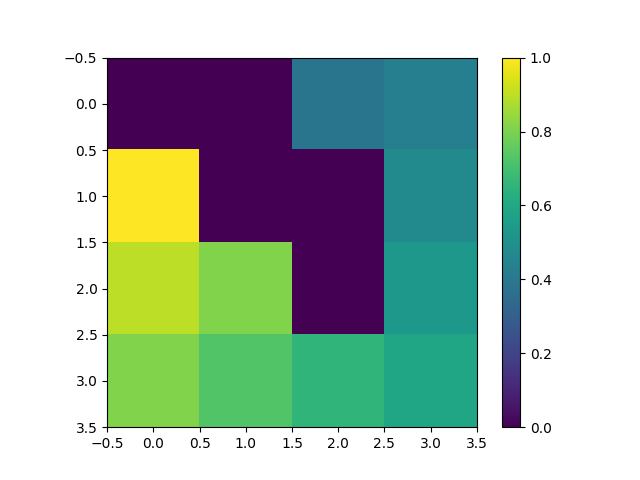
\includegraphics[width=.5\textwidth]{figures/sync_value_iteration_value_map.png}
  \caption{\label{fig:prob3_value_image_solution_for_value_iteration} Solution of value function color plot for a $4 \times 4$ map of the \texttt{FrozenLake-v0} environment.}
\end{figure}
\FloatBarrier

\begin{figure}[h]
  \centering
  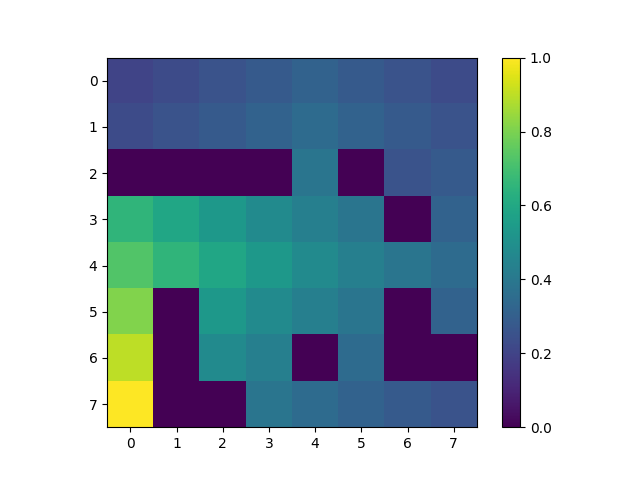
\includegraphics[width=.5\textwidth]{figures/8X8_sync_value_iteration_value_map.png}
  \caption{\label{fig:prob3_value_image_solution_for_value_iteration_8X8} Solution of value function color plot for a $8 \times 8$ map of the \texttt{FrozenLake-v0} environment.}
\end{figure}
\FloatBarrier


\item Which algorithm was faster, policy iteration or value iteration? Which took fewer iterations? Are there any differences in the value function? (2 pts)

\begin{solution}
Value-iteration was faster than policy iteration. \\
Value-iteration took fewer iterations than policy-iteration\\
There is no difference between the value function derived from two approaches: policy-iteration versus value-iteration
\end{solution}

\item Convert the optimal value function to the optimal policy. Show  the policy a grid of letters with ``U'', ``D'', ``L'', ``R'' representing the actions up, down, left, right respectively. See Figure~\ref{fig:prob2_example_policy} for an example of the expected output. (3 pts)

\begin{solution}
For 4x4 map: \\
LLRD \\
ULLD \\
ULLD \\
ULLL \\ \\
For 8x8 map: \\
DDDDDLLL \\
RRRRDLLL \\
LLLLDLRD \\
DLLLLLLD \\
DLLLLLLL \\
DLULLLLU \\
DLULLULL \\
RLLULLLL

\end{solution}

\item Implement \textbf{asynchronous policy iteration} using two heuristics:
\begin{enumerate}[1.]
\item The first heuristic is to sweep through the states in the order they are defined in the gym environment. Specifically, you will implement\\
\texttt{policy\_iteration\_async\_ordered()} in \texttt{deeprl\_hw1/rl.py}, writing the policy evaluation  step in \texttt{evaluate\_policy\_async\_ordered()}. 
\item The second heuristic is to choose a random permutation of the states at each iteration and sweep through all of them.  Specifically, you will implement\\
\texttt{policy\_iteration\_async\_randperm()} in \texttt{deeprl\_hw1/rl.py}, writing the policy evaluation  step in \texttt{evaluate\_policy\_async\_randperm()}. 
\end{enumerate}
Fill in the table below with the results for Deterministic-8x8-FrozenLake-v0: (5 pts)

\begin{center}
  \begin{tabular}{|c|c|c|c|}\hline
    {\bf Heuristic} & {\bf Time (ms)} & {\bf \shortstack{Policy \\ Improvement \\ Steps}} & {\bf \shortstack{Total \\ Policy \\ Evaluation \\ Steps}} \\ \hline
    Ordered & & & \\ \hline
    Randperm & & & \\ \hline
  \end{tabular}
\end{center}

\begin{solution}
\begin{center}
  \begin{tabular}{|c|c|c|c|}\hline
    {\bf Heuristic} & {\bf Time (ms)} & {\bf \shortstack{Policy \\ Improvement \\ Steps}} & {\bf \shortstack{Total \\ Policy \\ Evaluation \\ Steps}} \\ \hline
    Ordered & 17.26 & 13 & 91\\ \hline
    Randperm & 23.44 & 13 & 97\\ \hline
  \end{tabular}
\end{center}
\end{solution}

\item Implement \textbf{asynchronous value iteration} using two heuristics:
\begin{enumerate}[1.]
\item The first heuristic is to sweep through the states in the order they are defined in the gym environment. Specifically, you will implement\\
\texttt{value\_iteration\_async\_ordered()} in \texttt{deeprl\_hw1/rl.py}.
\item The second heuristic is to choose a random permutation of the states at each iteration and sweep through all of them.  Specifically, you will implement\\
\texttt{value\_iteration\_async\_randperm()} in \texttt{deeprl\_hw1/rl.py}.
\end{enumerate}
Fill in the table below with the results for Deterministic-8x8-FrozenLake-v0: (5 pts)

\begin{center}
  \begin{tabular}{|c|c|c|}\hline
    {\bf Heuristic} & {\bf Time(s)} & {\bf \# Iterations} \\ \hline
    Ordered & & \\ \hline
    Randperm & & \\ \hline
  \end{tabular}
\end{center}

\begin{solution}
\begin{center}
  \begin{tabular}{|c|c|c|}\hline
    {\bf Heuristic} & {\bf Time(ms)} & {\bf \# Iterations} \\ \hline
    Ordered & 4.896 & 13 \\ \hline
    Randperm & 4.81 & 10 \\ \hline
  \end{tabular}
\end{center}
\end{solution}

\item Write an agent that executes the optimal policy. Record the total cumulative discounted reward. Does this value match the value computed for the starting state? If not, explain why. (3 pts)

\begin{center}
  \begin{tabular}{|c|c|c|}\hline
    {\bf Env} & {\bf $V(s_0)$ Computed} & {\bf $V(s_0)$ Simulated}  \\ \hline
    4x4  & & \\ \hline
    8x8  & & \\ \hline
  \end{tabular}
\end{center}

\begin{solution}
\begin{center}
  \begin{tabular}{|c|c|c|}\hline
    {\bf Env} & {\bf $V(s_0)$ Computed} & {\bf $V(s_0)$ Simulated}  \\ \hline
    4x4  & 0.43046 & 0.43046 \\ \hline
    8x8  & 0.28242 & 0.28242 \\ \hline
  \end{tabular}
\end{center}
The value matche the value computed for the starting state.
\end{solution}

\end{enumerate}

\subsection*{Problem 2, Part II: Stochastic Environment (10 pt)}

In this section, we will use the stochastic versions of the FrozenLake environment. Answer the following questions for the maps
\texttt{Stochastic-4x4-FrozenLake-v0} and \\
\texttt{Stochastic-8x8-FrozenLake-v0}.

\begin{enumerate}[a)]
\item Using \textbf{synchronous value iteration}, find the optimal value function. Record
  the time taken for execution and the number of iterations required. Use a
  stopping tolerance of $10^{-3}$. Use $\gamma=0.9$. (2 pts)
\begin{center}
  \begin{tabular}{|c|c|c|}\hline
    {\bf Environment} & {\bf Time (ms)} & {\bf \# Iterations} \\ \hline
    Stochastic-4x4 & & \\ \hline
    Stochastic-8x8 & & \\ \hline
  \end{tabular}
\end{center}

\begin{solution}
\begin{center}
  \begin{tabular}{|c|c|c|}\hline
    {\bf Environment} & {\bf Time (ms)} & {\bf \# Iterations} \\ \hline
    Stochastic-4x4 & 3.86 & 29 \\ \hline
    Stochastic-8x8 & 14.97 & 26 \\ \hline
  \end{tabular}
\end{center}
\end{solution}

\item Plot the value function as a color map like in Part I. Is the
  value function different compared to the deterministic versions of
  the maps? (2 pts)
\begin{solution}
4X4: Figure~\ref{fig:prob3_value_image_solution_for_value_iteration_stochastic} \\
8X8: Figure~\ref{fig:prob3_value_image_solution_for_value_iteration_8X8_stochastic}
The values are different for stochastic as now we have 0.33 probability for doing the right motion and 0.66 probability of making error. In this case, the agent will learn the values in according to this distribution.
\end{solution}

\begin{figure}[h]
  \centering
  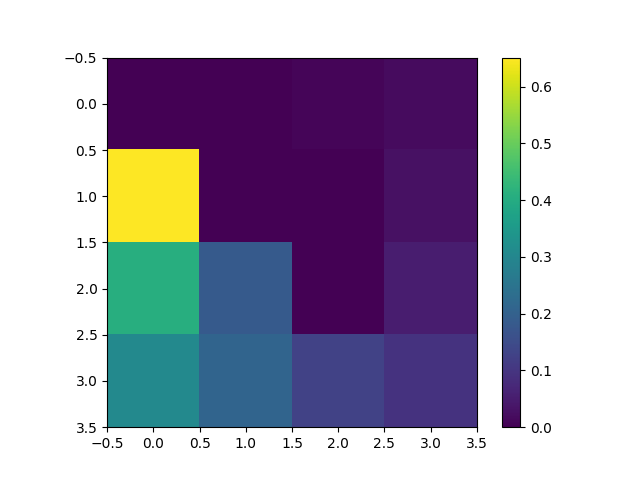
\includegraphics[width=.5\textwidth]{figures/stochastic_sync_value_iteration_value_map.png}
  \caption{\label{fig:prob3_value_image_solution_for_value_iteration_stochastic} Solution of value function color plot for a $4 \times 4$ map of the \texttt{FrozenLake-v0} environment.}
\end{figure}
\FloatBarrier

\begin{figure}[h]
  \centering
  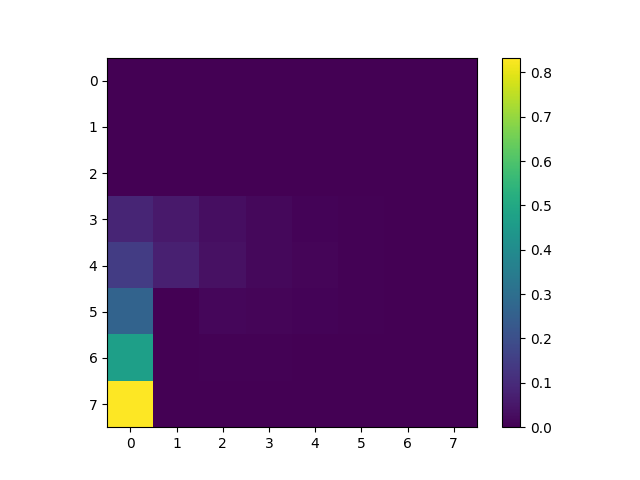
\includegraphics[width=.5\textwidth]{figures/stochastic_8X8_sync_value_iteration_value_map.png}
  \caption{\label{fig:prob3_value_image_solution_for_value_iteration_8X8_stochastic} Solution of value function color plot for a $8 \times 8$ map of the \texttt{FrozenLake-v0} environment.}
\end{figure}
\FloatBarrier
  
\item Convert this value function to the optimal policy and include it in the writeup. Does this optimal policy differ from the optimal policy in the deterministic map? If so, pick a state where the policy differs and explain why the action is different. (3 pts)
  
\begin{solution}
For 4x4 map: \\
LLRR \\
LLLR \\
LLLR \\
LLDD \\ \\
For 8x8 map: \\
URRRRLLL \\
UUUURUUD \\
LLLLLLRR \\
DDDDDLLR \\
LUULLLDU \\
LLRUULLR \\
LLRLLLLL \\
DLLRDLDD \\ \\
The optimal policy in stochastic map is different compared to deterministic map. For example: let us consider the state 3 in 4x4 map. In deterministic map, the optimal action is "DOWN" as it is the upper right corner and there is hole on the left and down is the only safe tile. Whereas, in stochastic map, the optimal action is "RIGHT". This ensures that the agent will move either down to only safe position with 0.33 probability and or stay in its location with 0.66 probability.
\end{solution}
  
\item Write an agent that executes the optimal policy. Run this agent $100$ times on the map and record the total cumulative discounted reward. Average the results. Does this value match the value computed for the starting state? If not explain why. (3 pts)
  
\begin{center}
  \begin{tabular}{|c|c|c|}\hline
    {\bf Env} & {\bf $V(s_0)$ Computed} & {\bf $V(s_0)$ Simulated}  \\ \hline
    4x4  &  &  \\ \hline
    8x8  &  &  \\ \hline
  \end{tabular}
\end{center}

\begin{solution}
\begin{center}
  \begin{tabular}{|c|c|c|}\hline
    {\bf Env} & {\bf $V(s_0)$ Computed} & {\bf $V(s_0)$ Simulated}  \\ \hline
    4x4  &  0.0206 &  0.024 \\ \hline
    8x8  &  0.000375 &  0.00041 \\ \hline
  \end{tabular}
\end{center}
As it is a stochastic environment, the convergence to exact values is very important. Here we are choosing tolerance of 0.001 as convergence criteria for bellman error. Hence, a difference in the order of $10^{-3}$ is justified here.
\end{solution}
  
\end{enumerate}


\subsection*{Problem 2, Part III: Custom Heuristic for Asynchronous DP (8 pt)}

In this part, you will design a custom heuristic for asynchronous value iteration\\
(\texttt{value\_iteration\_async\_custom()}) to try to beat the heuristics previously defined (although this is not a requirement for full points). A potential idea for the heuristic might be to sweep through the entire state space ordered by e.g. distance to goal. You do not need to systemically sweep through the entire state space in your design (but you can do so if you so choose).

\begin{enumerate}[a)]
\item Fill in the table below with the results for asynchronous value iteration using your custom heuristic. Compare against the previous heuristics. Since the previous heuristics did do a systemic sweep through the entire state space, you can compare against them by measuring the number of individual state updates. You can calculate this for the old heuristics by taking \# Iterations and multiplying it by the size of the state space. (5 pts)
\begin{center}
  \begin{tabular}{|c|c|c|}\hline
    {\bf Env} & {\bf Time (s)} & {\bf \# Individual State Updates} \\ \hline
    Deterministic-4x4 & & \\ \hline
    Deterministic-8x8 & & \\ \hline
    Stochastic-4x4    & & \\ \hline
    Stochastic-8x8    & & \\ \hline
    %Custom & & & \\ \hline
  \end{tabular}
\end{center}

\begin{solution}
\begin{center}
  \begin{tabular}{|c|c|c|c|c|}\hline
    {\bf Env} & {\bf Time} & {\bf \# Ind State} & {\bf \# Ind State} & {\bf \# Ind State} \\
    {\bf} & {\bf (ms)} & {\bf Updates} & {\bf Updates} & {\bf Updates} \\ 
    {\bf} & {} & {\bf custom} & {\bf Ordered} & {\bf RandPerm} \\ \hline
    D-4x4 & 0.808 & 57 & 72 & 102 \\ \hline
    D-8x8 & 6.75 & 603 & 208 & 144 \\ \hline
    S-4x4 & 6.6 & 420 & 352 & 416 \\ \hline
    S-8x8 & 25.59 & 1575 & 352 & 368 \\ \hline
    %Custom & & & \\ \hline
  \end{tabular}
\end{center}
\end{solution}

\item Provide an intuitive description of your heuristic (max 250 word). (3 pts)

\begin{solution}
I have implemented a priority queue (decreasing order) for states. Before constructing the queue, I check if the state is terminal and add the state to queue (with zero key value) only if the state is not terminal. In each loop, I pop the first element from queue, update its state value using bellman equation and push the state back in the queue with key value as:
\begin{enumerate}
\item $\Delta = -|old\_value(state) - new\_value(state)|$ if $\Delta > tolerance$
\item zero if $\Delta < tolerance$. In this case, I also increase the counter (think of it as number of times the state got visited)and use it in priority queue. For states with same priority value get arranged with decreasing counter values.
\end{enumerate} 
My stopping criteria is that all the states in the queue have values converged. I am maintaining a counter to check if convergence is achieved.
\end{solution}

\end{enumerate}



\section*{Problem 3 (25 pts)} 

For this problem, assume the MDP has finite state and action spaces. Let $V^\pi(s)$ be the value of policy $\pi$ when starting at state $s$. That is:
\[
V^\pi(s) := \mathbb{E}_\pi \left[ \sum_{k=0}^\infty \gamma^k r_{t+1+k} \mid s_t = s \right]
\]
A policy $\pi$ is called {\it deterministic} if for all states $s\in S$, there exists an action $a\in A$ such that $\pi(a|s) = 1$.

\begin{itemize}
\item[(a)] Assume $\gamma < 1$. Show that for all policies $\pi$ and states $s \in S$, the value function $V^\pi(s)$ is well-defined, i.e., (i) the infinite sum $\sum_{k=0}^\infty \gamma^kr_{t + 1 + k}$ converges even if the episode never terminates and (ii) the outer expectation $\mathbb{E}_\pi[\cdot]$ is well-defined. (5 pts)

\begin{solution}
(i) As this is an example of finite MDP, the number of states transitions $\tau \in T$ are finite. Also let $r_{\tau}$ represents the reward corresponding to $\tau$ transition. Hence we can split the infinite sum equation as:
\begin{align}
\hspace{3em} &\sum_{k=0}^\infty \gamma^k r_{t + 1 + k} = \sum_{\tau \in T} R_{\tau} \\
where,& \hspace{3em} R_{\tau} = r_{\tau}\times (\gamma^{\tau_1} +\gamma^{\tau_2} + \gamma^{\tau_3} + ... + \gamma^{\tau_m})\\
and& \hspace{3em} 0 \leq \tau_1 \leq \tau_2 \leq \tau_3 \leq ... \leq \tau_m \\ \\
\end{align}

If we can show that each term in above summation ($R_{\tau}$) converges than $\sum_{k=0}^\infty \gamma^k r_{t + 1 + k}$ will also converge. \\
I will use ratio rule to show convergence. The two consecutive terms in expression for $R_{\tau} = r_{\tau}\times (\gamma^{\tau_1} +\gamma^{\tau_2} + \gamma^{\tau_3} + ... + \gamma^{\tau_m})$ as $r_{\tau}\times\gamma^{\tau_m}$ and $r_{\tau}\times\gamma^{\tau_{m+1}}$.\\ \\
Hence, the ratio between two consecutive terms is: \\ 
$
\frac{r_{\tau}\times\gamma^{\tau_m}}{r_{\tau}\times\gamma^{\tau_{m+1}}} = \gamma^{\tau_{m+1} - \tau_{m}} < 1 \hspace{3em}$
as $\gamma < 1$ and $\tau_{m+1} > \tau_{m}\\
$

(ii) $\mathbb{E}_\pi[\cdot] = \sum_{a \in A} \pi(a|s) \times [\cdot]$ \\
As this is deterministic policy, the summation will reduce to one term for which the probability is 1. As the term, for which the expectation is being calculated, is converging, the absolute value of the term will converge and hence $\mathbb{E}_\pi[\cdot]$ is well defined.
\end{solution}


\item[(b)] Show that for every state $s\in S$, there exists a deterministic policy $\pi_s$ that is optimal for that state $s$ amongst deterministic policies (i.e., $V^{\pi_s}(s) \ge V^{\pi}(s)$ for every deterministic policy $\pi$). (3 pts)

\begin{solution}
For every state $s \in S$, we can select a deterministic policy $\pi$ that gives the maximum value for that state $s$ and call it the optimal policy for that state $s$. Hence, \\
$ \pi_s(s) = argmax_\pi V^\pi (s)$ \\ 
$ \pi_s(s) = argmax_\pi \ \max_{a \in A} (\pi(a|s)\times \sum_{r, s'}p(s'|a,s)(r(s'|a,s) + \gamma V^{\pi}(s')))$
\end{solution}

\item[(c)] Given state-optimal deterministic policies $\pi_s$ as defined in part (b), write down a deterministic policy $\pi^*$ that is optimal for all states among deterministic policies (i.e., $V^{\pi^*}(s) \ge V^{\pi}(s)$ for all states $s$ and deterministic policies $\pi$). (3 pts)

\begin{solution}
$ \forall s \in S$\\
$\pi^*(s) = \pi_s(s)$ \\
$V^{\pi^*}(s) = V^{\pi_s}(s) \ge V^{\pi}(s)$
\end{solution}

\end{itemize}


\begin{itemize}

\item[(d)] Assume that the discount factor is 1.  Give an example MDP and policy where the value function is infinite, i.e., the value of the infinite sum diverges. (2 pt)

\begin{solution} 
We can use the example from problem 1 itself where the agent needs to go to coffee location. If $\gamma = 1$ and there is  positive reward for every action, the agent will keep moving in the grid and collecting reward, hence the value function will be infinite.
\end{solution}

\item[(e)] Specify a reasonable criterion which can be used for deciding whether one infinite-valued policy is superior to another. (3  pts)

\begin{solution}
\begin{enumerate}
\item Given start and goal positions, we will run the agent with given infinite valued policies and see the success rates for multiple runs. Here success is defined as reaching the goal position. The policy with higher success rate will be superior to other
\item Given same success rate, the policy with higher average cumulative reward will be superior
\end{enumerate}
\end{solution}

\item[(f)] Assume that the discount factor is 1. Specify an MDP with multiple states and actions that has an infinite-valued optimal policy according to this criterion. Specify the policy and show that it is optimal. (4 pts)

\begin{solution}
Figure~\ref{fig:prob3_MDP}\\
G is terminal state. \\
$S_1$ is start. \\
\begin{center}
  \begin{tabular}{|c|c|c|c|}\hline
    {\bf Previous State} & {\bf Action} & {\bf Next State} & {\bf Reward} \\ \hline
    $S_1$ & "$S1S2$" & $S_2$ & +1 \\ \hline
    $S_2$ & "$S2S1$" & $S_1$ & -1 \\ \hline
    $S_2$ & "$S2G$" & $G$ 	& +10\\ \hline
    $S_2$ & "$S2S3$" & $S_3$ & $-\infty$\\ \hline
    $S_3$ & "$S3S4$" & $S_4$ & +1\\ \hline
    $S_4$ & "$S4S3$" & $S_3$ & +1\\ \hline
  \end{tabular}
\end{center}
$\pi_1:$
\begin{center}
  \begin{tabular}{|c|c|c|}\hline
    {\bf Previous State} & {\bf Action} & {\bf Value} \\ \hline
    $S_1$ & "$S1S2$" & 11 \\ \hline
    $S_2$ & "$S2G$" & +10 \\ \hline
    $S_3$ & "$S3S4$" & $\infty$\\ \hline
    $S_4$ & "$S4S3$" & $\infty$\\ \hline
  \end{tabular}
\end{center}

$\pi_2:$
\begin{center}
  \begin{tabular}{|c|c|c|}\hline
    {\bf Previous State} & {\bf Action} & {\bf Value} \\ \hline
    $S_1$ & "$S1S2$" & 0 \\ \hline
    $S_2$ & "$S2S1$" & 0 \\ \hline
    $S_3$ & "$S3S4$" & $\infty$ \\ \hline
    $S_4$ & "$S4S3$" & $\infty$\\ \hline
  \end{tabular}
\end{center}

$\pi_3:$
\begin{center}
  \begin{tabular}{|c|c|c|}\hline
    {\bf Previous State} & {\bf Action} & {\bf Value} \\ \hline
    $S_1$ & "$S1S2$" & 1 \\ \hline
    $S_2$ & "$S2S3$" & 0 \\ \hline
    $S_3$ & "$S3S4$" & $\infty$ \\ \hline
    $S_4$ & "$S4S3$" & $\infty$ \\ \hline
  \end{tabular}
\end{center}

$\pi_1$ is the optimal infi$\pi_1$ is the superior of all three policies as this is the only policy that reaches goal position and is the optimal policy of all three policy.
\end{solution}
\begin{figure}[h]
  \centering
  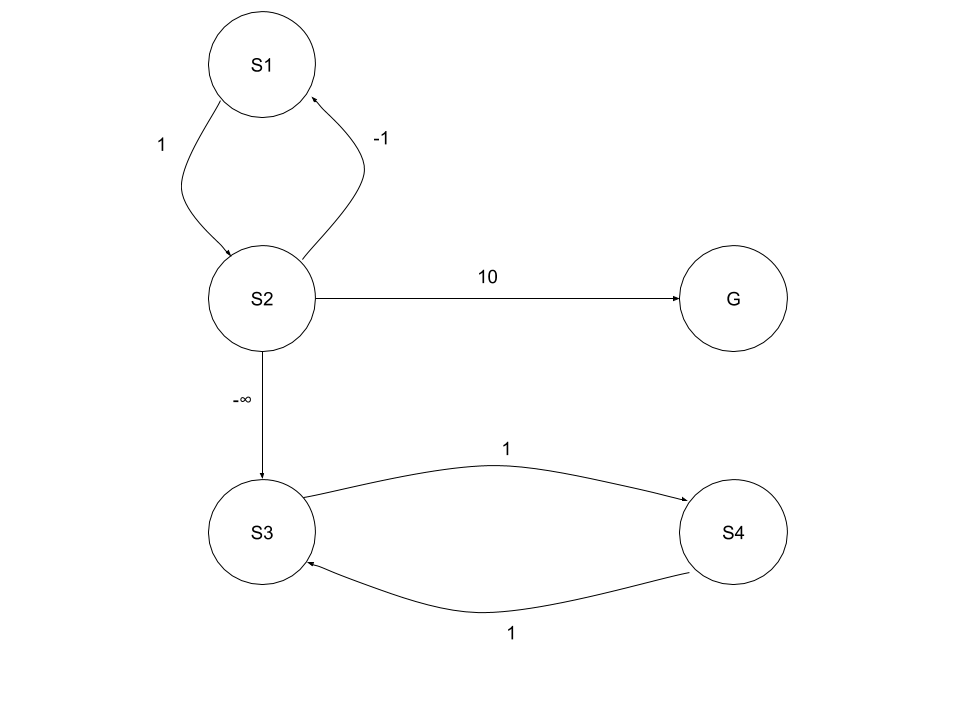
\includegraphics[width=1\textwidth]{figures/MDP.png}
  \caption{\label{fig:prob3_MDP} MDP}
\end{figure}
\FloatBarrier


\item[(g)] Assume that the discount factor is 1. Specify an MDP which has multiple infinite-valued policies for which there exists no clear criterion for deciding which is superior. Specify those policies and explain your reasoning. (4 pts)

\begin{solution}
Figure~\ref{fig:prob3_MDP2}\\
G is terminal state. \\
$S_1$ is start. \\
\begin{center}
  \begin{tabular}{|c|c|c|c|}\hline
    {\bf Previous State} & {\bf Action} & {\bf Next State} & {\bf Reward} \\ \hline
    $S_1$ & "$S1S2$" & $S_2$ & +1 \\ \hline
    $S_2$ & "$S2S1$" & $S_1$ & -1 \\ \hline
    $S_2$ & "$S2S3$" & $S_3$ & $-\infty$\\ \hline
    $S_3$ & "$S3S4$" & $S_4$ & +1\\ \hline
    $S_4$ & "$S4S3$" & $S_3$ & +1\\ \hline
    $S_4$ & "$S4G$" & $G$ & 0\\ \hline
  \end{tabular}
\end{center}
$\pi_1:$
\begin{center}
  \begin{tabular}{|c|c|c|}\hline
    {\bf Previous State} & {\bf Action} & {\bf Value} \\ \hline
    $S_1$ & "$S1S2$" & 0 \\ \hline
    $S_2$ & "$S2S1$" & 0 \\ \hline
    $S_3$ & "$S3S4$" & $\infty$ \\ \hline
    $S_4$ & "$S4S3$" & $\infty$\\ \hline
  \end{tabular}
\end{center}

$\pi_2:$
\begin{center}
  \begin{tabular}{|c|c|c|}\hline
    {\bf Previous State} & {\bf Action} & {\bf Value} \\ \hline
    $S_1$ & "$S1S2$" & 1 \\ \hline
    $S_2$ & "$S2S3$" & 0 \\ \hline
    $S_3$ & "$S3S4$" & $\infty$ \\ \hline
    $S_4$ & "$S4S3$" & $\infty$ \\ \hline
  \end{tabular}
\end{center}

Here, none of the two infinite valued policy result into reaching goal position so we can not clearly say which one is superior.
\end{solution}

\begin{figure}[h]
  \centering
  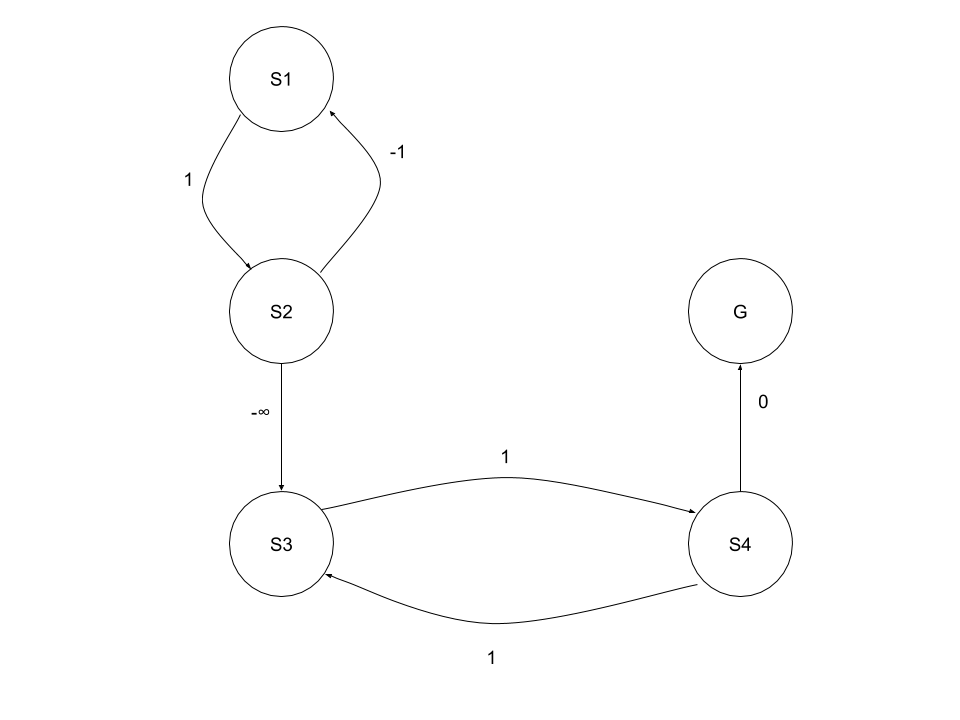
\includegraphics[width=1\textwidth]{figures/MDP2.png}
  \caption{\label{fig:prob3_MDP2} MDP\_2}
\end{figure}
\FloatBarrier

\item[(h)] Give a class of infinite-horizon MDPs where $\gamma=1$ but every stationary policy has finite value. (1 pts)

\begin{solution}
Any MDP where we have cycle between two states with equal and opposite reward of transition between them, would fall into this criteria. Here the value will be finite but it will be infinite horizon MDP.
\end{solution}
\end{itemize}

\end{document}